% Insert after VI-D. Requires graphicx. Copy figures/ next to the manuscript.
\subsection{Timing Fidelity and Simulation Cost}
We validate the operation-level scheduler against a separately implemented
capacity-one FIFO dispatcher driving NetSquid 1.1.7 timed
\texttt{QuantumProcessor} instructions. Both paths receive the same arrivals
and configured durations. The native path dispatches its next request only on
the processor's program-completion event; it does not reuse QuCl's scheduling
code or computed completion timestamps. Equal-time arrivals are submitted as
a batch in input order. The comparison includes idle, saturated, simultaneous,
bursty, and completion-boundary arrivals (including offsets of $\pm1$ ns),
BSMs of 1.6 ms, corrections of 0.5 and 0.05 ms, and variable-duration correction
workloads. Across 120 workloads and 2,500 requests, the maximum absolute
start, completion, and waiting-time differences are all 0 ns. Replaying 500
R/B requests from 12 actual mixed-protocol runs also gives 0 ns maximum error.
This establishes timing equivalence for the specified atomic FIFO model;
it does not validate physical device durations or gate-level noisy evolution.

For simulation cost, we execute finite mixed Swap--Teleport batches of
1, 4, 8, 16, 32, and 64 sessions with a request interval of 0.8 ms, at
R--B background offered loads of 0 and 0.70. Each condition has one warmup
and ten measured repetitions in shuffled order. All runs retain native memory
noise, production event logging, and the full background-traffic drain.
Runtime includes state initialization, ns-3 startup/configuration, federation,
and shutdown, but excludes build/import time, offline independent-reference
validation, and result-file writing. All repeated traces are identical within
each condition and pass packet, resource, clock, and quantum-state validation.
The error bars in Fig.~\ref{fig:timing-cost}(b) are 95\% bootstrap intervals
over runtime repetitions, not over network workloads. These measurements
characterize finite-batch cost on a fixed topology, rather than isolated IPC
overhead or arbitrary-topology scalability.

At 64 sessions, mean total simulation runtimes are 1.17 [1.00, 1.40] and 1.50 [1.41, 1.61] s at offered loads 0 and 0.70, respectively. The corresponding synchronization-round counts are 418 and 817, and bidirectional IPC line counts are 2381 and 4110. Counts include setup and the complete traffic drain.

\begin{figure*}[t]
\centering
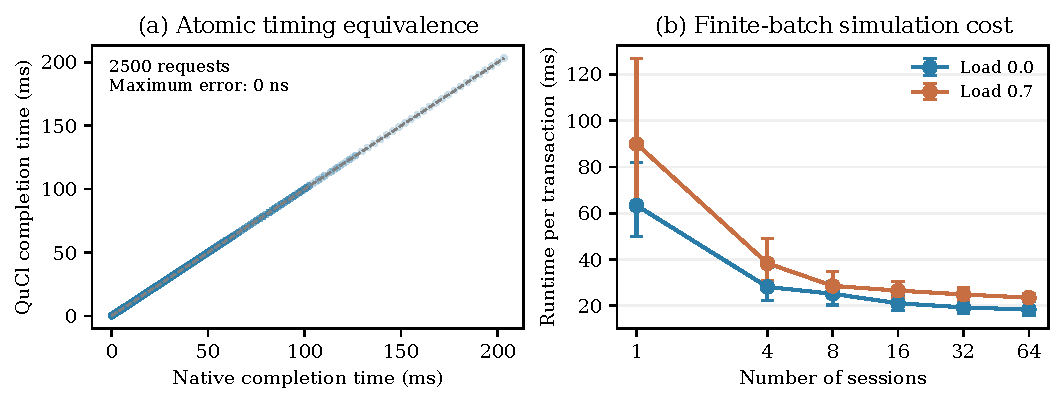
\includegraphics[width=\textwidth]{figures/fig7-timing-cost.pdf}
\caption{Additional validation. (a) Atomic completion timing against an
independent dispatcher using native timed instructions. (b) Mean simulation
runtime per completed transaction, with 95\% repetition-bootstrap intervals.
Offline reference validation and file writing are excluded.}
\label{fig:timing-cost}
\end{figure*}
